\section{Apache Kafka}
%http://de.slideshare.net/tim.lossen.de/eventstream-processing-with-kafka
%http://de.slideshare.net/charmalloc/developingwithapachekafka-29910685

Nach der Vorstellung von Apache Storm wird in diesem Kapitel Apache Kafka näher gebracht. Zu Beginn wird eine Kurzübersicht gegeben, um anschließend die Bewertungskriterien zu erläutern. Apache Kafka wird von Rao in \citeint{kafka:Proposal} als verteiltes publish-subscribe Nachrichtensystem für die Verarbeitung hoher Mengen an fließenden Daten. Am 04.07.2011 wurde der Apache Incubation-Prozess aufgenommen und am 23.10.2012 wurde Apache Kafka qualifiziert \citeint{kafka:IncubationStatus}. Ursprünglich wurde Apache Kafka von der Firma LinkedIn \citeint{linkedin} um auf die eingehenden unterschiedlichen hohen Datenmengen der Webseiten von LinkedIn Zugang zu bekommen und zu verarbeiten \citeint{kafka:Proposal}.

\begin{table}[htbp]
	\centering
		\begin{tabular}{@{}ll@{}} \toprule
			\textbf{Faktum} & \textbf{Beschreibung} \\ \midrule
			Hauptentwickler & Jay Kreps, Neha Narkhede, Jun Rao \\
			Stabile Version & 0.8.1.1 vom 29.04.2014 \\ 
			Entwicklungsstatus &  Aktiv \\
			Entwicklungsversion & 0.8.2, 0.9.0 \\
			Sprache & Scala, Java, Python \\
			Betriebssystem & Platformübergreifend (Microsoft Windows mit Cygwin Umgebung) \\
			Lizenz & Apache License version 2.0 \\
			Webseite & \citeint{kafka:home} \\
			Quelltext & \citeint{kafka:GitHubApacheMirror} \\			
			\bottomrule			
		\end{tabular}
	\caption{Kurzübersicht Apache Kafka}
	\label{tab:vorkafka}
\end{table}

Die Architektur von Apache Kafka besteht aus einem Kafka Server, den \textit{Producern} und den \textit{Consumern}. Der Server stellt als \textit{Broker} die Verbindungen zwischen einem \textit{Producer} und einem \textit{Consumer} her. In einem \textit{Broker} werden \textit{Topics} registriert. Ein spezifischer Nachrichtenstrom kann durch Angabe eines \textit{Topic} bereitgestellt oder abgefragt werden. Der \textit{Producer} hält eine Liste von Verbindungen zu \textit{Brokern}. Nachrichten werden von \textit{Producern} an \textit{Broker}, wie in einem \textit{Push}-System gesendet. Bei Absturz eines \textit{Brokers} wird ein bestehender \textit{Broker} zum \textit{Master} gewählt, der zuerst aus einer Anfrage auf Aktivität antwortet. Ein \textit{Consumer} zieht Nachrichten von einem \textit{Broker}, wie in einem \textit{Pull}-System. Aktives Warten auf Dateneingang in einem "`long poll"', einem permanenten Abfragen eines \textit{Brokers} durch den \textit{Consumer}, kann durch Übergabe von Parametern in der \textit{Consumer}-Abfrage blockiert werden. Der Nachrichtenstrom stellt in einem \textit{Consumer} eine \textit{Iterator}-Schnittstelle bereit. Sobald Nachrichten eintreffen, können weiterführende Operationen ausgeführt werden. Um eine Last zu verteilen, kann ein \textit{Topic} in Partitionen aufgeteilt werden. Eine Nachricht besteht aus einem Schlüssel und einem Wert. Der Nachrichtenschlüssel kann je nach Strategie z.B. per Zufall auf bestimmte Partitionen zugeordnet werden. Partitionen sind auf Host-Maschinen in  einem Kafka-Cluster verteilt. Ein \textit{Topic} sollte in einem produktiven Einsatz die gleiche Anzahl an \textit{Threads} wie Partitionen haben. Bei geringerer Anzahl von \textit{Threads} als \textit{Topics}, entstehen Wartezeiten für \textit{Topics}. \textit{Topics} können in diesem Fall die Arbeit nicht unmittelbar starten, sondern müssen auf einen \textit{Thread}, der bereit wird, warten. Mit Kommandozeilen-Werkzeugen kann ein \textit{Rebalance} der Partitionen von \textit{Topics} in einem Kafka-\textit{Cluster} angestoßen werden. \citelit[S. 2, Kap. 3]{apache:kafka:kreps2011kafka}

\begin{figure}[htb!]
\centering
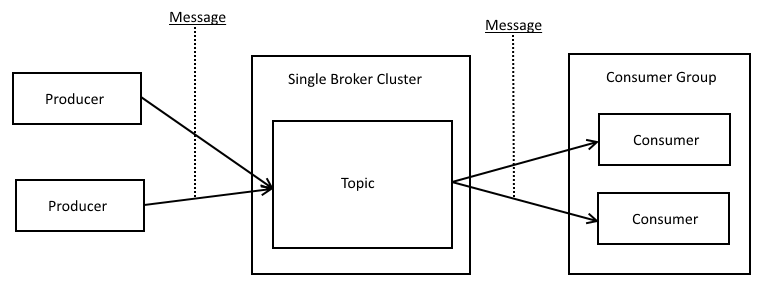
\includegraphics[width=1.0\textwidth]{bilder/kafkaDesign.png}
\caption{Apache Kafka Architektur - Single Broker Cluster
\label{fig:kafkaDesign}}
\end{figure}

Abbildung \ref{fig:kafkaDesign} zeigt ein Beispiel mit einem \textit{Single Broker Cluster} als Server. Das Kafka-Cluster kann auch aus mehreren \textit{Brokern} bestehen. Die Installationsanleitung in Anhang \ref{section:kafkainstall} zeigt eine Konfiguration für ein \textit{Single Broker Cluster}. Für ein \textit{Multi Broker Cluster} werden separate Konfigurationen der Kafka-Maschinen und ein Apache Zookeeper-Cluster benötigt. In der Abbildung \ref{fig:kafkaDesign} werden Nachrichten an das \textit{Topic} von Zwei \textit{Producern} gesendet. Aus der \textit{Consumer Group} holen Zwei \textit{Consumer} Nachrichten aus dem \textit{Topic} ab. Für die Koordination der Nachrichten greifen der \textit{Server}, die \textit{Producer} und die \textit{Consumer} im Hintergrund auf Apache Zookeeper zu. Für die horizontale Skalierung kann ein Apache Zookeeper Cluster genutzt werden. In einem Kafka-Cluster können maximal 255 Knoten existieren. Pro Konfiguration muss jeder Knoten eine eigene Identität unter der \textit{Broker-Id} festgelegt bekommen. Mehrere Knoten mit gleicher Identität führen zu einem unvorhersagbaren \textit{Cluster}-Verhalten. \citelit[S. 28]{garg2013apache}

Sobald Nachrichten von \textit{Consumern} in einem Kafka-Cluster empfangen werden, werden diese lokal innerhalb einer Apache Zookeeper-Maschine im Dateisystem gespeichert. In einem \textit{Consumer} werden die Nachrichten mit einem iterativen Zähler im \textit{Offset} gespeichert. Durch die Angabe des \textit{Offset} ist es möglich Nachrichten von einer \textit{Topic}-Partition ab einer bestimmten \textit{Offset}-Position abzuholen. Beim Speichern der Nachrichten nutzt Apache Kafka die \textit{zero-copy}-Optimierung \citeint{ibmZeroCopy}. Dabei wird die Nachricht in den Linux Page Cache einmalig geschrieben. Weitere Abfragen der Nachrichten werden vom Page Cache geliefert. Durch die zero-copy-Optimierung werden 4 context-switches pro Abfrage in einem Prozess reduziert. \citeint[Kap. 4.3]{kafka:documentation}

In Kafka wird die Reihenfolge von Nachrichten, die von einer \textit{Topic}-Partition abgeholt wird, garantiert. Die Reihenfolge von unterschiedlichen Partitionen kann allerdings abweichen und wird nicht garantiert. In Apache Kafka können Nachrichten mit der \textit{Gzip\footnote{Kompressionswerkzeug: gzip -- \url{http://www.gzip.org/}}}-Anwendung oder der \textit{Snappy\footnote{Kompressionsbibliothek: snappy -- \url{https://code.google.com/p/snappy/}}}-Bibliothek komprimiert werden. Nachrichten werden von Kafka nach einer Verarbeitung in einem \textit{Consumer} abschließend nicht gelöscht. Durch das einstellbare \gls{glo:sla} ist es möglich Nachrichten erst nach einer definierten Zeitspanne zu löschen. In einem \textit{Consumer}-Ausfall ist es durch diese Technik möglich, Nachrichten mit einem neuen bzw. bestehenden \textit{Consumer} erneut abzufragen, also Nachrichten neu einzuspielen. Dennoch sind bei der Übernahme Nachrichten-Duplikate möglich. Eine Anwendung die Kafka einsetzt und mit Duplikaten umgehen muss, muss eine Logik zur Erkennung von Duplikaten bereitstellen.
So wird beim Einsatz von mehreren \textit{Consumern} die Datenkapazität vervielfacht. Nachrichten sind verloren, falls ein \textit{Broker} mit nicht abgeholten Nachrichten ausfällt. \citelit[S. 4, Kap. 3.3]{apache:kafka:kreps2011kafka}

Aus dem Apache Kafka Archiv \citeint{kafka:GitHubApacheMirror} wurde ein Beispiel für die Verwendung von \textit{Producer} und \textit{Consumer} im Anhang unter dem Quelltext \ref{lst:kafkaProducer} und \ref{lst:kafkaConsumer} abgelegt. Beide Klassen erben von der Java \textit{Thread}-Klasse. In einer externen Klasse können beide erweiterten \textit{Threads} instanziiert und mit der \textit{start}-Methode ausgeführt werden. Im \textit{Producer}-Quelltext wird innerhalb der \textit{run}-Methode in einer Schleife eine Nachricht dauerhaft an einen übergebenen \textit{Topic} gesendet. Im \textit{Consumer}-Quelltext wird ebenfalls in der \textit{run}-Methode über ein \textit{Mapping} der \textit{KafkaStream} für das übergebene \textit{Topic} geholt und über den \textit{ConsumerIterator}, solange Nachrichten eintreffen, die Nachrichten in der Konsole ausgegeben. In beiden Implementierungen wird zuvor eine Konfiguration für das Kafka-Cluster gesetzt. Im Quelltext \ref{lst:kafkaProducer} und \ref{lst:kafkaConsumer} liegt eine hierarchische Benennung vor. Die Klasse KafkaStream liegt z.B. im Namensraum "`kafka.consumer.KafkaStream"'. Die Hierarchie wird durch den Punkt abgetrennt. Spezifiert wird von links nach rechts. Beim Synchronisieren zwischen Producer und Consumer werden über Apache Zookeeper Watcher Listener Konfigurationen aktualisiert.

\begin{table}[ht!]
	\centering
		\begin{tabular}{@{}ll@{}} \toprule
			\textbf{Kriterium} & \textbf{Bewertung} \\ \midrule
			Architektur & Strukturierte Peer-to-Peer-Architektur \\
			Prozesse und Threads & Client-Server Cluster, Actice Push-Pull-Modell \\
			Kommunikation & TCP-basiert mit Apache Zookeeper \\
			Namenssystem & Hierarchische Benennung \\
			Synchronisierung & Apache Zookeeper Watcher \\
			Pipelining und Materialisierung & Publishing als Consumer \\
			Konsistenz und Replikation & Replikation \\
			Fehlertoleranz & Fail-Fast Strategie unter Supervision \\ %CRC removal of bad CRCs -> self healing?
			Sicherheit & Nur eigene Maßnahmen \\
			Erweiterung & Eigenentwicklung und Community-Beiträge \\
			Qualität & At-least-once delivery, time-based \gls{glo:sla} 7 Tage \\
			\bottomrule			
		\end{tabular}
	\caption{Bewertung Apache Kafka}
	\label{tab:bewkafka}
\end{table}

Apache Kafka kann \textit{Topic}-Partitionen replizieren. Mit einem \textit{Replication}-Faktor kann die Anzahl der Replikate in der Konfiguration für einen \textit{Topic} eingestellt werden. Das erste registrierte \gls{glo:isr} bekommt die führende Rolle. Weitere Replikate übernehmen den Status des \textit{Follower}, dem Folgenden. Falls der führende \gls{glo:isr} abstürzt, wird durch den Algorithmus \textit{PacificA} \citelit{pacifica} aus den \textit{Followern} der nächste führende \gls{glo:isr} bestimmt. \citeint[Kap. 4.7]{kafka:documentation}

Da Apache Kafka auf einem Publish-Subscribe-Verfahren aufbaut ist die Wiederbenutzung bzw. Weitergabe von Nachrichten nur unter Angabe eines weiteren \textit{Topic} möglich. Dafür sind mindestens ein weiterer \textit{Publisher} und \textit{Consumer} zu implementieren. Aggregatoren und Operatoren, sowie es unter dem Referenzmodell Aurora/Borealis angeboten wird, kann unter Apache Kafka in der Hochsprache Scala oder Java in einem Producer entwickelt werden. Auch in der Sicherheit fehlen noch Anforderungen zur Authentifizierung und Verschlüsselung innerhalb des Kafka-Clusters \citeint{kafka:security}. Erweiterungen für das Monitoring werden über \gls{glo:jmx} angeboten. Eine Integration in ein Monitoringsystem wie Nagios kann mit dem Java JMX Nagios Plugin\footnote{Java JMX Nagios Plugin: check\_jmx -- \url{http://exchange.nagios.org/directory/Plugins/Java-Applications-and-Servers/check\_jmx/details}} erfolgen.

%http://de.slideshare.net/JayKreps1/i-32858698
%log aggregation: http://engineering.linkedin.com/distributed-systems/log-what-every-software-engineer-should-know-about-real-time-datas-unifying

In diesem Kapitel wurde die Installation und ein Beispielanwendung für den Austausch von Nachrichten gezeigt. Auf spezielle Eigenschaften wie das zero-copy \citelit{ibmZeroCopy}, Parallelisierung und Replikation wurde eingegangen. Außerdem wurden die Bewertungskriterien aus Tabelle \ref{tab:bewkafka} für Apache Kafka erläutert. Im nächsten Kapitel wird nun Apache Flume vorgestellt.


% jkreps / benchmark-commands.txt: https://gist.github.com/jkreps/c7ddb4041ef62a900e6c